\documentclass[15pt]{article}
\usepackage[utf8]{inputenc}
\pagestyle{plain}
\usepackage{amsmath, amssymb, amsfonts, amsthm, mathtools,mathrsfs}
\usepackage[
top    = 2.75cm,
bottom = 2.55cm,
left   = 3.00cm,
right  = 3.00cm]{geometry}
\usepackage{graphicx}
\usepackage{xcolor}

% \pagecolor[RGB]{18,18,18} %blackish
% \color[rgb]{0.9, 0.9, 0.9} %greyish

\usepackage{bm}
\usepackage{hyperref}
\usepackage{titlesec}
\usepackage{tocloft}
\usepackage{caption}
\usepackage{subcaption}
\usepackage[none]{tocbibind}
\usepackage{float}
\usepackage{fancyhdr}

\titleformat*{\subsection}{\normalfont}
\graphicspath{ {./EE229 images/} }
\definecolor{- }{RGB}{124,131,253}
\definecolor{blue}{RGB}{150,186,255}
\setcounter{secnumdepth}{5}
\setcounter{tocdepth}{1}

\pagestyle{fancy}
\fancyhf{}
\renewcommand{\headrulewidth}{0pt}
\renewcommand{\footrulewidth}{0.4pt}
\fancyfoot[R]{ADI}
\fancyfoot[L]{\thepage}

\renewcommand{\b}[1]{\begin{#1}}
\newcommand{\e}[1]{\end{#1}}
\renewcommand{\i}{\item{}}
\newcommand{\tb}[1]{\textbf{#1}}
\renewcommand{\thefigure}{}
\renewcommand{\cfttoctitlefont}{\Huge}

\b{document}
   \b{center}
       \vspace*{12cm}
       \tb{{\Huge EE229 Short Notes}}
       
       \vspace{0.9cm}
       \tb{\LARGE Aditya Byju}
            
       \vspace{0.5cm}
       \large {\tb{Course Professor:} Prof. Sibi Raj B. Pillai\\
       \tb{Ref:} Prof's slides, Signals and Systems by  Alan V. Oppenheim\\
       The untuned mind receives no signal from the universe\hspace{0.05cm}!}
       
       \vspace{0.5cm}
       \tb{Signal Processing - 1}
       
       \vspace{0.5cm}
       September 2021
            
       \vspace{0.8cm}
    \e{center}
\thispagestyle{empty}

\newpage
\tableofcontents
\addtocontents{toc}{\vspace{0.2cm}}

\newpage
\phantomsection
\section*{\color{- }Introduction}
\addcontentsline{toc}{section}{\large\color{- }Introduction}

\b{itemize}
    \i All the concepts described apply to both continuous-time and discrete-time signals unless otherwise mentioned
    \i \tb{continuous-time signals} - the independent variable is continuous, and thus these signals are defined for a continuum of values of the independent variable
    \i \tb{discrete-time signals} - defined only at discrete times, i.e. for these signals, the independent variable takes on only a discrete set of values
    \i The total energy over the time interval $t_1 \leq t \leq t_2$ in a continuous-time signal $x(t)$ is defined as\\
    \b{equation*}
      ||x||^2 =  \int_{t_1}^{t_2} |x(t)|^2 \,dt 
    \e{equation*}
    \i The total energy over the time interval $n_1 \leq n \leq n_2$ in a discrete-time signal $x[n]$ is defined as\\
    \b{equation*}
       \sum_{n\hspace{0.05cm}=\hspace{0.05cm}n_1}^{n_2} |x[n]|^2 
    \e{equation*}
    \i Some definitions:
    \b{itemize}
        \item[$-$] \tb{amplitude scaling of signals:} $y(t)= \alpha\hspace{0.05cm} x(t), ~\alpha \in \mathbb{R} ~\text{or}~ \alpha \in \mathbb{C}$ 
        \item[$-$] \tb{time-scaling:} $y(t)=  x(\alpha \hspace{0.05cm}t), ~\alpha \in \mathbb{R}$  
        \item[$-$] \tb{time-shift:} $y(t)=  x(t - \tau), ~\tau \in \mathbb{R}$  
        \item[$-$] \tb{time-reversal:} $y(t)=  x(-t)$
        \item[$-$] \tb{DC offset:} $y(t)= \alpha + x(t)$  
    \e{itemize}
\e{itemize}

\phantomsection
\section*{\color{- }Different types of signals}
\addcontentsline{toc}{section}{\large\color{- }Different types of signals}

\b{itemize}
    \i \tb{periodic signal} - a signal $x(t)$ having the property that there is a positive value of $T$ for which:\\
    \b{equation*}
       x(t) = x(t + T) 
    \e{equation*}
    The fundamental period is the smallest positive value of $T$
    \i \tb{even and odd signals} - signals satisfying the equations $x(-t) = x(t)$ and $x(-t) = -x(t)$ respectively
    \i \tb{discrete-time unit impulse or unit sample} is defined as:\\
    \b{equation*}
       \delta[n] = \begin{cases}
				0,~ n \neq 0\\
				1,~ n = 0
			\end{cases} 
    \e{equation*}
    \i \tb{discrete-time unit step} is defined as:\\
    \b{equation*}
       u[n] = \begin{cases}
				0,~ n < 0\\
				1,~ n \geq 0
			\end{cases} 
    \e{equation*}
    \i \tb{continuous-time unit impulse (Dirac measure)} is defined as:\\
    \b{equation*}
       \delta (t) = \begin{cases}
				0,~ t \neq 0\\
				\infty,~ t = 0
			\end{cases} 
    \e{equation*}
    \i \tb{continuous-time unit step} is defined as:\\
    \b{equation*}
       u(t) = \begin{cases}
				0,~ t < 0\\
				1,~ t \geq 0
			\end{cases} 
    \e{equation*}
    \i Relation between the 2 above signals:\\
    \b{equation*}
       \delta(t) =  \frac{du(t)}{dt} 
    \e{equation*}
    \i \tb{energy and power signals} - energy signal has finite energy and zero power whereas power signal has finite power and infinite energy
\e{itemize}

\phantomsection
\section*{\color{- }Systems}
\addcontentsline{toc}{section}{\large\color{- }Systems}

\b{itemize}
    \i \tb{system} - any process that produces an output signal in response to an input signal
    \i \tb{memoryless system} - output for each value of the independent variable at a given time is dependent on the input at only that same time
    \i The concept of {\color{blue}memory} in a system corresponds to the presence of a mechanism that retains or stores information about input values at times other than the current time. In many physical systems, memory is directly associated with the storage of energy.
    \i A system is said to be {\color{blue}invertible} if distinct inputs lead to distinct outputs
    \i If a system is invertible, then an {\color{blue}inverse system} exists that, when cascaded with the original system, yields an output that is equal to the input to the first system
    \i A system is {\color{blue}causal} if the output at any time depends on values of the input at only the present and past times. Such a system is often referred to as being {\color{blue}nonanticipative,} as the system output does not anticipate future values of the input.
    \i All memoryless systems are causal, since the output responds only to the current value of the input
    \i A {\color{blue}stable system} is one in which small inputs lead to responses that do not diverge. Stability of physical systems generally results from the presence of mechanisms that dissipate energy. If the input to a stable system is bounded, then the output must also be bounded and therefore cannot diverge.
    \i Conceptually, a system is {\color{blue}time-invariant} if the behaviour and characteristics of the system are fixed over time. Specifically, a system is time-invariant if a time shift in the input signal results in an identical time shift in the output signal.
    \i A {\color{blue}linear system,} in continuous or discrete time, is a system that possesses the important property of {\color{blue}superposition.} Let $y_1(t)$ be the response of a continuous-time system to an input $x_1(t)$, and let $y_2(t)$ be the output corresponding to the input $x_2(t)$. Then the system is linear if:
    \b{itemize}
        \item[$-$] the response to $x_1(t) + x_2(t)$ is $y_1(t) + y_2(t)$. (\tb{additivity property})
        \item[$-$] The response to $ax_1(t)$ is $ay_1(t)$, where $a$ is any complex constant. (\tb{scaling or homogeneity property})
    \e{itemize}
    \i A system can be linear without being time-invariant, and it can be time-invariant without being linear
    \i A direct consequence of the superposition property is that, for linear systems, an input which is zero for all time results in an output which is zero for all time
    \i {\color{blue}Pure all-pass system} has impulse response $\delta (t)$
    \i Some common systems:
    \begin{figure}[H]
    \centering
    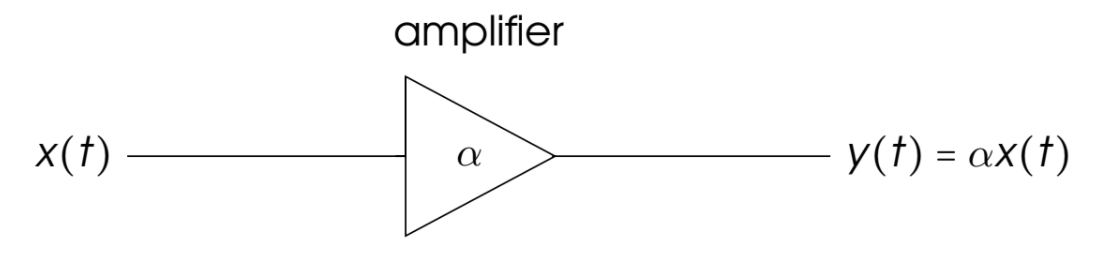
\includegraphics[width=11cm]{EE229 images/Amplifier.png}
    \end{figure}
    \begin{figure}[H]
    \centering
    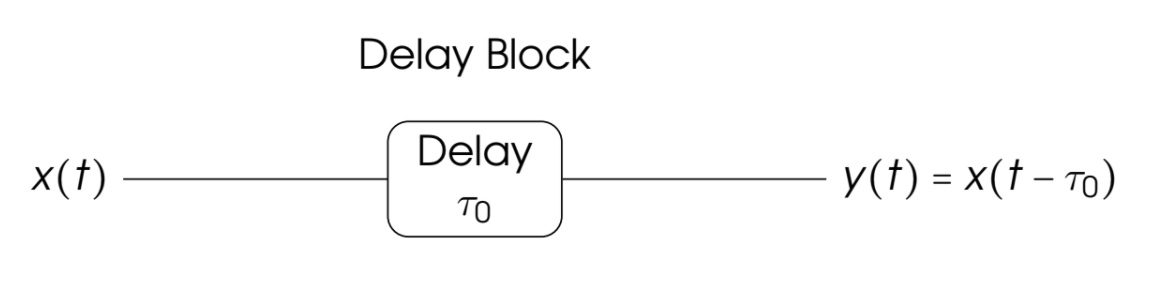
\includegraphics[width=11cm]{EE229 images/Delay block.png}
    \end{figure}
    \i Generalized echo system:
    \b{equation*}
       y(t) = \sum_{l\hspace{0.05cm} = \hspace{0.05cm}0}^{L} \alpha_l x(t - \tau_l)
    \e{equation*}
    \begin{figure}[H]
    \centering
    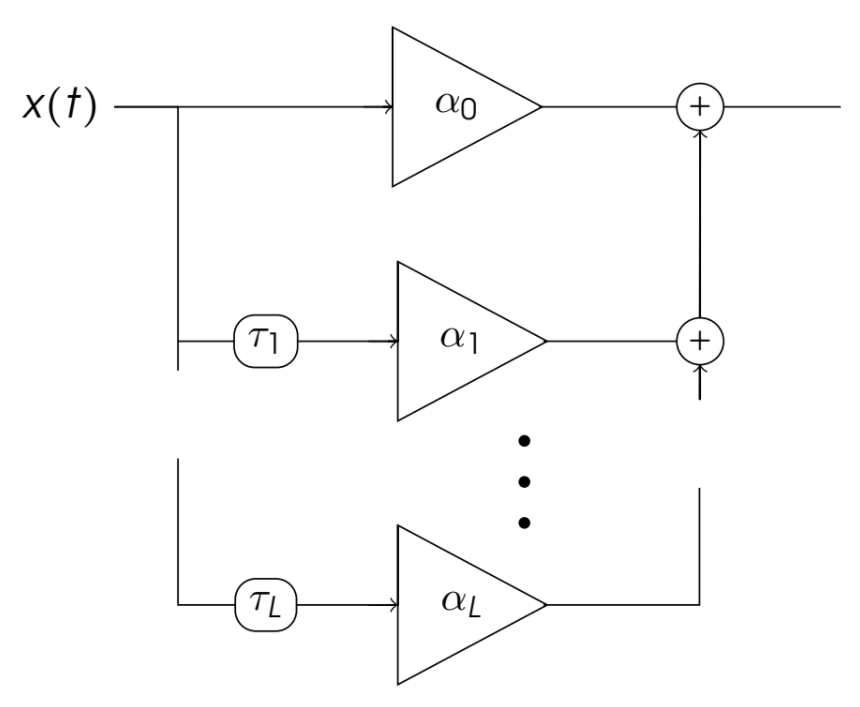
\includegraphics[width=11cm]{EE229 images/Generalized echo system.png}
    \end{figure}
\e{itemize}

\phantomsection
\section*{\color{- }Linear time-invariant systems}
\addcontentsline{toc}{section}{\large\color{- }Linear time-invariant systems}

\b{itemize}
    \i \tb{linear time-invariant (LTI) system} - systems that are both linear and time-invariant
    \i {\color{blue}Convolution sum} or {\color{blue}superposition sum} of two discrete-time LTI systems $x[n]$ and $h[n]$:
    \b{equation*}
       x[n]*h[n] = \sum_{k\hspace{0.05cm}=\hspace{0.05cm}-\infty}^{\infty} x[k]h[n-k]
    \e{equation*}
    \i {\color{blue}Convolution integral} or {\color{blue}superposition integral} of two continuous-time LTI systems $x(t)$ and $h(t)$:
    \b{equation*}
       x(t)*h(t) = \int_{-\infty}^{\infty} x(\tau)h(t - \tau)d\tau
    \e{equation*}
    \i Convolution is commutative, distributive and associative:
    \b{equation*}
       x(t)*h(t) = h(t)*x(t)
    \e{equation*}
    \b{equation*}
       x(t)*[h_1(t) + h_2(t)] = x(t)*h_1(t) + x(t)*h_2(t)
    \e{equation*}
    \b{equation*}
       x(t)*[h_1(t)*h_2(t)] = [x(t)*h_1(t)]*h_2(t)
    \e{equation*}
    \i Impulse response of a system ($h(t)$) and its inverse system ($h_1(t)$) satisfy:
    \b{equation*}
       h(t)*h_1(t) = \delta(t)
    \e{equation*}
    \i A continuous-time LTI system is stable if the impulse response is absolutely integrable, i.e., if:
    \b{equation*}
       \int_{-\infty}^{\infty} |h(\tau)|d\tau < \infty
    \e{equation*}
    \i A discrete-time LTI system is stable if the impulse response is absolutely summable, i.e., if:
    \b{equation*}
       \sum_{k \hspace{0.05cm}=\hspace{0.05cm} -\infty}^{\infty} |h[k]| < \infty
    \e{equation*}
    \i Zero-order hold and first-order hold:
    \begin{figure}[H]
    \centering
    \begin{minipage}{.5\textwidth}
    \centering
    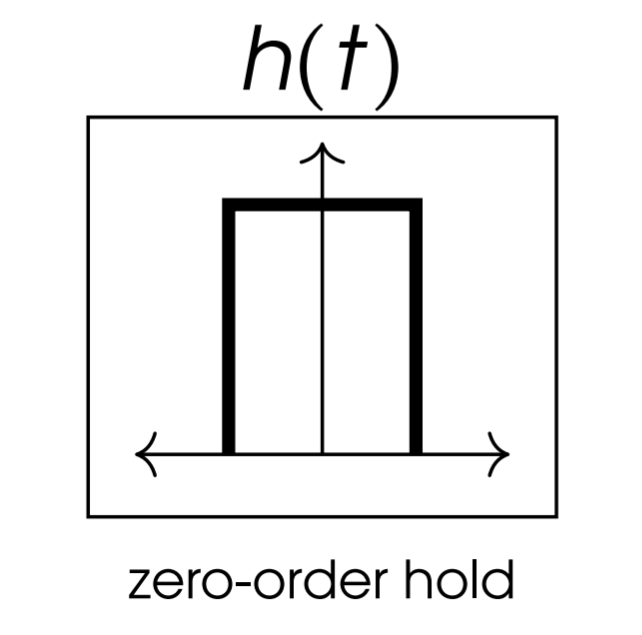
\includegraphics[width=.5\linewidth]{EE229 images/Zero-order hold.png}
    \label{fig:test1}
    \end{minipage}%
    \begin{minipage}{0.5\textwidth}
    \centering
    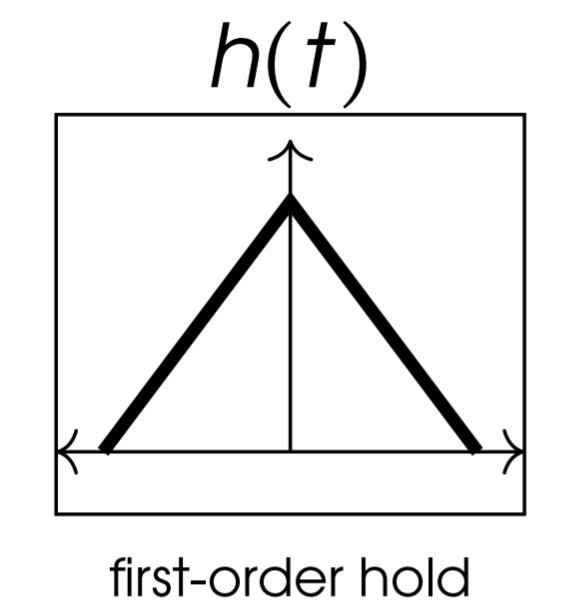
\includegraphics[width=.45\linewidth]{EE229 images/First-order hold.png}
    \label{fig:test2}
    \end{minipage}
    \end{figure}
    \i \tb{digital interpolation} - upsampling followed by digital convolution
    \i \tb{cubic interpolation} - this type of interpolation gives rise to a piecewise cubic function that interpolates a set of data points and guarantees smoothness at the data points
\e{itemize}

\phantomsection
\section*{\color{- }Fourier series representation of continuous-time signals}
\addcontentsline{toc}{section}{\large\color{- }Fourier series representation of continuous-time signals}

\b{itemize}
    \i An even function can be represented as:
    \b{equation*}
       f(x) = \sum_{m \hspace{0.05cm}\geq\hspace{0.05cm} 0}^{} a_m\cos(\frac{2\pi}{T}mx) ,~\text{for}~ \frac{-T}{2} \leq x  \leq \frac{T}{2}
    \e{equation*}
    \i An odd function can be represented as:
    \b{equation*}
       f(x) = \sum_{m \hspace{0.05cm}\geq \hspace{0.05cm}1}^{} b_m\sin(\frac{2\pi}{T}mx) ,~\text{for}~ \frac{-T}{2} \leq x  \leq \frac{T}{2}
    \e{equation*}
    \i Functions $g_1,~g_2$ such that $\langle g_1,~g_2 \rangle = 0$ for $t \in T$ is said
    to be orthogonal in $T$.
    \i A representation of a periodic signal as a combination of complex exponentials of discrete frequencies, which are multiples of the fundamental frequency of the signal, is known as the Fourier series representation of the signal
    \b{equation*}
       x(t) = \alpha_0 + \sum_{n\hspace{0.05cm}\geq \hspace{0.05cm}1}^{} a_n\cos(\frac{2\pi}{T_d}nT) + \sum_{n\hspace{0.05cm} \geq \hspace{0.05cm}1}^{} b_n\sin(\frac{2\pi}{T_d}nT) 
    \e{equation*}
    \b{equation*}
      = \alpha_0 + \sum_{n\hspace{0.05cm} \geq\hspace{0.05cm} 1}^{} a_n\frac{(e^{j\frac{2\pi}{T_d}nt} + e^{-j\frac{2\pi}{T_d}nt})}{2} + \sum_{n \hspace{0.05cm}\geq \hspace{0.05cm}1}^{} b_n\frac{(e^{j\frac{2\pi}{T_d}nt} - e^{-j\frac{2\pi}{T_d}nt})}{2j}
    \e{equation*}
    \b{equation*}
      = \sum_{m \hspace{0.05cm}\in \hspace{0.05cm}\mathbb{Z}}^{} \alpha_m e^{j\frac{2\pi}{T_d}mt}
    \e{equation*}
    \b{equation*}
      \text{where} ~\alpha_m = \frac{a_m - b_m}{2},~ m \in \mathbb{Z}^{+}~ \text{and}~ \alpha_m = \frac{a_{|m|} + b_{|m|}}{2}, m \in \mathbb{Z}^{-}
    \e{equation*}
    \b{equation*}
      \alpha_m = \frac{\langle~ x(t),~ e^{j\frac{2\pi}{T_d}mt}~ \rangle}{T_d} = \frac{1}{T_d} \int_{-\frac{T_d}{2}}^{\frac{T_d}{2}} x(t)e^{-j\frac{2\pi}{T_d}mt}dt 
    \e{equation*}
    \i \tb{Theorem:} No two continuous functions in $[-\frac{T}{2}, ~\frac{T}{2}]$  will have all the Fourier series coefficients the same
    \i \tb{Lemma:} Let $f(t)$ be a signal locally integrable in $[-\frac{T}{2}, ~\frac{T}{2}]$ , if the Fourier series coefficients $\alpha_m = 0,$ identically $\forall m \in Z,$ then $f(t) = 0,$
whenever it is continuous at $t$
    \i \tb{Properties of continuous-time Fourier series}\\
    \hspace*{20pt}If the Fourier series coefficients of $x(t)$ are denoted by $a_k$, we will use the notation:
    \b{equation*}
      \hspace{0.8cm}x(t) \xleftrightarrow{\mathcal{~FS~}} a_k
    \e{equation*}
    \b{itemize}
        \item[$-$] \tb{Linearity:}\\
        \b{equation*}
            \text{If}~~ x(t) \xleftrightarrow{\mathcal{~FS~}} a_k~ ~and~~y(t) \xleftrightarrow{\mathcal{~FS~}} b_k, ~ \text{then}
        \e{equation*}
        \b{equation*}
            z(t) = Ax(t) + By(t) \xleftrightarrow{\mathcal{~FS~}} c_k = Aa_k + Bb_k
        \e{equation*}
        \item[$-$] \tb{Time shifting:}\\ 
        \b{equation*}
            \text{If}~~ x(t) \xleftrightarrow{\mathcal{~FS~}} a_k, ~ \text{then}
        \e{equation*}
        \b{equation*}
            x(t-t_0) \xleftrightarrow{\mathcal{~FS~}} e^{-(j\frac{2\pi}{T}kt_0)}a_k
        \e{equation*}
        \item[$-$] \tb{Time reversal:}\\
        \b{equation*}
            \text{If}~~ x(t) \xleftrightarrow{\mathcal{~FS~}} a_k, ~ \text{then}
        \e{equation*}
        \b{equation*}
            x(-t) \xleftrightarrow{\mathcal{~FS~}} a_{-k}
        \e{equation*}
        \item[$-$] \tb{Time scaling:}\\
        \b{equation*}
            x(t) = \sum_{k \hspace{0.05cm}=\hspace{0.05cm} -\infty}^{\infty} a_k e^{(j\frac{2\pi}{T}kt)}
        \e{equation*}
        \b{equation*}
            x(\alpha t) = \sum_{k\hspace{0.05cm} = \hspace{0.05cm}-\infty}^{\infty} a_k e^{(j\frac{2\pi}{T}k\alpha t)}
        \e{equation*}
        \item[$-$] \tb{Multiplication:}\\
        \b{equation*}
            \text{If}~~ x(t) \xleftrightarrow{\mathcal{~FS~}} a_k~ ~\text{and}~~y(t) \xleftrightarrow{\mathcal{~FS~}} b_k, ~ \text{then}
        \e{equation*}
        \b{equation*}
            z(t) = x(t)y(t) \xleftrightarrow{\mathcal{~FS~}} c_k = \sum_{l \hspace{0.05cm}= \hspace{0.05cm}-\infty}^{\infty} a_l b_{k-l}
        \e{equation*}
        \item[$-$] \tb{Conjugation:}\\
        \b{equation*}
            \text{If}~~ x(t) \xleftrightarrow{\mathcal{~FS~}} a_k, ~ \text{then}
        \e{equation*}
        \b{equation*}
            x^*(t) \xleftrightarrow{\mathcal{~FS~}} a^*_{-k}
        \e{equation*}
    \e{itemize}
    \i \tb{Parseval's relation for continuous-time periodic signals:}
    \b{itemize}
        \item[$-$] If $x(t) = \sum_{m  \in  \mathbb{Z}}^{} \beta_m \phi_m t~$ with  $\langle \phi_m,~\phi_n \rangle = \delta [m-n]$ in $\frac{-T}{2} \leq x  \leq \frac{T}{2}$ , then:
    \e{itemize}
    \b{equation*}
            \int_{-\frac{T}{2}}^{\frac{T}{2}} |x(t)|^2 dt = \sum_{m\hspace{0.05cm}\in \hspace{0.05cm} \mathbb{Z}}^{} |\beta_m|^2
    \e{equation*}
    \i The total average power in a periodic signal equals the sum of the average powers in all of its harmonic components:
    \b{equation*}
            \frac{1}{T} \int_{-\frac{T}{2}}^{\frac{T}{2}} |x(t)|^2 dt = \sum_{m\hspace{0.05cm}\in \hspace{0.05cm} \mathbb{Z}}^{} |\alpha_m|^2
    \e{equation*}
    \i A function $h(t)$ is integrable if $ \int_{\mathbb{R}}^{} |h(t)|dt < \infty$
    \i \b{equation*}
            sinc(\theta) = \frac{\sin(\pi \theta)}{\pi \theta} 
    \e{equation*}
    \begin{figure}[H]
    \centering
    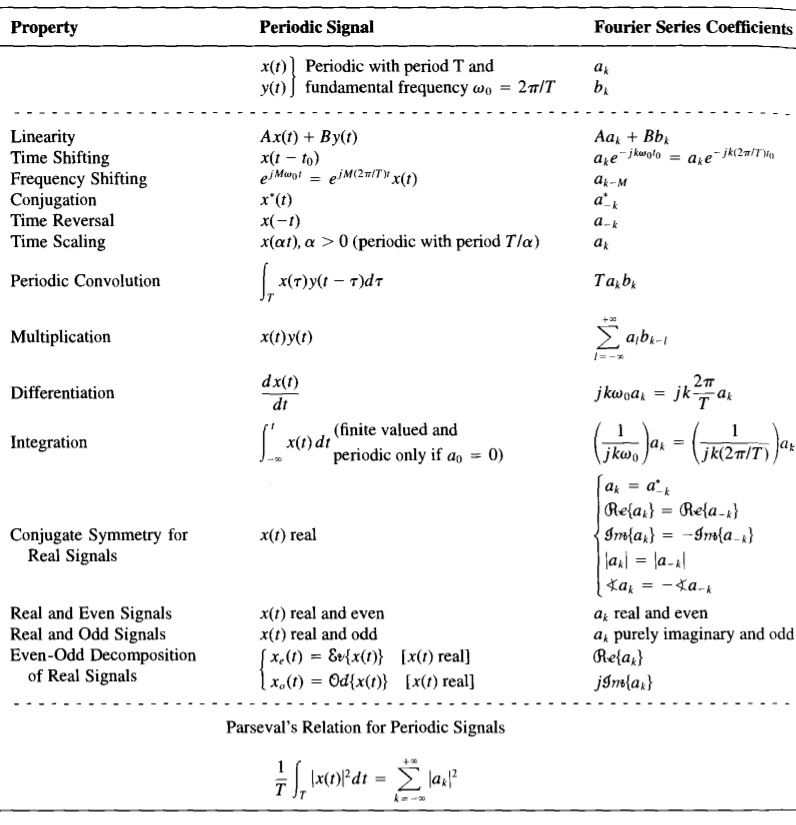
\includegraphics[width=15cm]{EE229 images/Properties of continuous-time fourier series.png}
    \caption{Properties of continuous-time Fourier series}
    \end{figure}
\e{itemize}

\phantomsection
\section*{\color{- }Fourier transforms}
\addcontentsline{toc}{section}{\large\color{- }Fourier transforms}

\b{itemize}
    \i The {\color{blue} Fourier transform} is a mathematical function that decomposes a waveform, which is a function of time, into the frequencies that make it up. The equation of Fourier transform ${H(f)}$ of a signal $x(t)$ is:\\
    \b{equation*}
           H(f) = \int_{\mathbb{R}}^{} x(t) e^{-(j2\pi ft)}dt
    \e{equation*}
    \i The properties of the Fourier transform are:\\
    \begin{figure}[H]
    \centering
    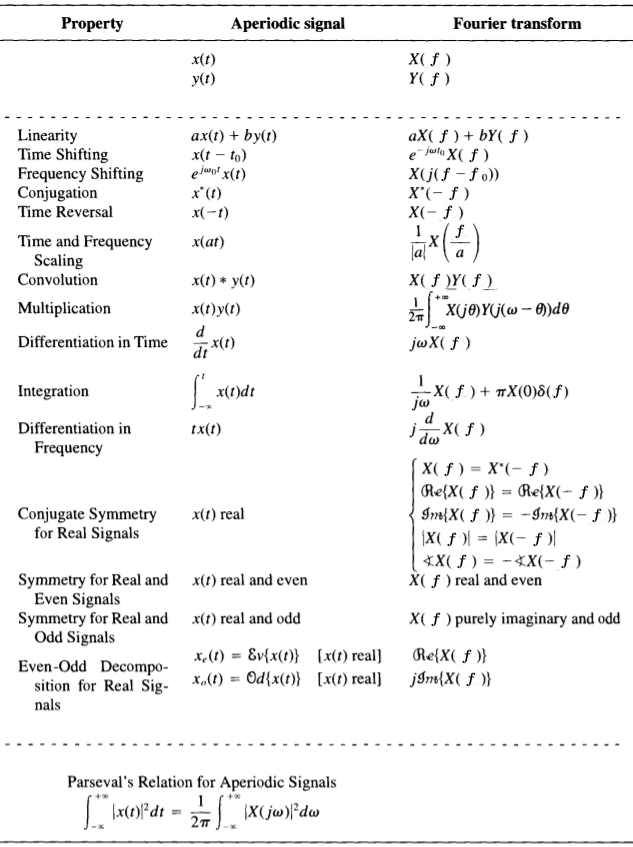
\includegraphics[width=15cm]{EE229 images/Properties of the fourier transform.png}
    \caption{Properties of the Fourier transform}
    \end{figure}
    \i \tb{Poisson summation formula:} For an integrable $x(t)$ with Fourier transform $H(f)$ - 
    \b{equation*}
           \sum_{n\hspace{0.05cm} \in\hspace{0.05cm} \mathbb{Z}}^{}x(t - nT) = \sum_{m \hspace{0.05cm} \in\hspace{0.05cm} \mathbb{Z}}^{} \alpha_m e^{(\frac{2\pi}{T} mt)},
    \e{equation*}\\
    \hspace{2cm}at points of continuity of the LHS, where
    \b{equation*}
           \alpha_m = \frac{1}{T} H(\frac{m}{T}), ~ m \in \mathbb{Z}
    \e{equation*}
    \vspace*{0.3cm}
    \i \b{equation*}
         e^{(-\pi t^2)} \xleftrightarrow{\mathcal{~FT~}}  e^{(-\pi f^2)} 
    \e{equation*}
    \vspace*{0.3cm}
    \i \b{equation*}
         g_\delta (t) = \frac{1}{\sqrt{\delta}} e^{(-\pi \frac{t^2}{\delta})} \xleftrightarrow{\mathcal{~FT~}}  e^{(-\pi f^2 \delta)} = G_\delta (f) ,~ \delta > 0 
    \e{equation*}
    \vspace*{0.3cm}
    \i \b{equation*}
          \lim_{\delta \downarrow 0}g_\delta (t) = \delta(t) ~ ~\rightarrow~~{\color{blue}\text{Impulse or Dirac measure}}
    \e{equation*}
    \vspace*{0.3cm}
    \i \b{equation*}
         \lim_{\delta \downarrow 0}G_\delta (f) = \mathbb{I}_{\{f\in \mathbb{R}\}} ~ ~\rightarrow~~{\color{blue}\text{DC value}}
    \e{equation*}
    \vspace*{0.3cm}
    \i The {\color{blue}Inverse Fourier transform} is given by:\\
    \b{equation*}
           x(t) = \int_{\mathbb{R}}^{} H(f) e^{(j2\pi ft)}df
    \e{equation*}\\
    where $H(f)$ is the Fourier transform of signal $x(t)$
    \i \tb{Poisson sum:} Fourier transform (Generalized) of an impulse train:
    $$ \sum_{n\hspace{0.05cm}\in\hspace{0.05cm}\mathbb{Z}} \delta(t-nT)  \xrightleftharpoons[]{F.T.} \sum_{m\hspace{0.05cm}\in\hspace{0.05cm}\mathbb{Z}} \frac{1}{T}\delta(f-\frac{m}{T})$$
    \i \tb{Dual FS formula:} 
    $$ \sum_{n\hspace{0.05cm}\in\hspace{0.05cm}\mathbb{Z}} X(f+n\beta) \xrightleftharpoons[]{I.F.T.} \sum_{m\hspace{0.05cm}\in\hspace{0.05cm}\mathbb{Z}} \frac{1}{\beta}x(\frac{m}{\beta})\delta(t-\frac{m}{\beta}) $$
    \i \tb{Shannon's reconstruction formula:}
    \b{equation*}
           x(t) = \sum_{m\hspace{0.05cm}\in\hspace{0.05cm}\mathbb{Z}} x(\frac{m}{\beta}) \hspace{0.1cm} sinc (\beta t-m)
    \e{equation*}
    \i \tb{Parseval's relation:}
    \b{equation*}
           \int_{\mathbb{R}} x(t)y^*(t)dt = \int_{\mathbb{R}} X(f)Y^*(f)df
    \e{equation*}
    \b{equation*}
           \int_{\mathbb{R}} |x(t)|^2dt = \int_{\mathbb{R}} |X(f)|^2df
    \e{equation*}
    \i Wireless communication bandwidths:
    \begin{figure}[H]
    \centering
    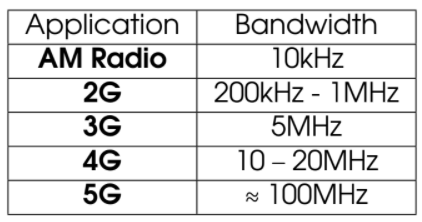
\includegraphics[width=5.5cm]{EE229 images/Wireless communication bandwidths.png}
    \end{figure}
\e{itemize}

\phantomsection
\section*{\color{- }Dirac's formalisms}
\addcontentsline{toc}{section}{\large\color{- }Dirac's formalisms}

\b{itemize}
    \i \tb{Def:} Dirac Delta is defined as a non-negative unit area operator such that:
    $$ \int_{\mathbb{R}} x(t)\delta(t)dt=x(0),~~~\text{whenever} ~x(0^+)=x(0^-)=x(0)$$
    \i Fourier transform and inverse for Diracs:
    $$ \delta(t) \xrightleftharpoons[]{F.T.} \mathbb{I}_{\{f\hspace{0.05cm}\in\hspace{0.05cm}\mathbb{R}\}} $$
    $$  \mathbb{I}_{\{t\hspace{0.05cm}\in\hspace{0.05cm}\mathbb{R}\}} \xrightleftharpoons[]{F.T.} \delta(f) $$
\e{itemize}    

\phantomsection
\section*{\color{- }Advanced concepts}
\addcontentsline{toc}{section}{\large\color{- }Advanced concepts}

\b{itemize}
    \i \tb{Inverse DTFT:} given samples $x[n],~n\in\mathbb{Z}$, having a DTFT $\hat{X}(f),~-\frac{1}{2}\leq f\leq\frac{1}{2}$:
    $$ x[n]=\int_{-\frac{1}{2}}^{\frac{1}{2}} \hat{X}(f)e^{(j 2 \pi f n )}$$
    \i \tb{Discrete Fourier transform (DFT):} 
    $$ X[k] = \hat{X} \bigg [\frac{k}{N}\bigg ] = \sum_{n\hspace{0.05cm}=\hspace{0.05cm}0}^{N-1}x[n] e^{(-j2\pi \frac{k}{N}n)} $$
    \i \tb{Matrix form of DFT:} 
    $$ \text{DFT:    }~~\overline{X}=F\hspace{0.05cm}\overline{x}$$
    $$ \text{where F }= \begin{bmatrix}
                        \alpha_{0}^{0} & \alpha_{0}^{1} & \alpha_{0}^{2} & \ldots & \alpha_{0}^{M}\\
                        \alpha_{1}^{0} & \alpha_{1}^{1} & \alpha_{1}^{2} & \ldots & \alpha_{1}^{M}\\
                        \alpha_{2}^{0} & \alpha_{2}^{1} & \alpha_{2}^{2} & \ldots & \alpha_{2}^{M}\\
                        . & . & . & \ldots & .\\
                        . & . & . & \ldots & .\\
                        . & . & . & \ldots & .\\
                        \alpha_{M}^{0} & \alpha_{M}^{1} & \alpha_{M}^{2} & \ldots & \alpha_{M}^{M}
                        \end{bmatrix} $$
    $$ \text{here } \alpha = e^{(-j\frac{2\pi}{N})},~~\alpha_i = \alpha^i~(\text{for} ~
    0\leq i\leq N-1),~~M=N-1 $$ 
    \tb{Proposition:} 
    $$F^HF=N\mathbb{I}_N$$
    \i \tb{Circular convolution ($\circledast$):} let $x_c[n]=\sum_{i\hspace{0.05cm}\in\hspace{0.05cm}\mathbb{Z}}x[n+iN] ~\rightarrow ~ x_c[i] = x[i+N]$ for $-N\leq i \leq -1$, then:
    $$ x_c[n] \circledast h[n] = \sum_{n\hspace{0.05cm}=\hspace{0.05cm}0}^{N-1} h[n] x_c[k-n] $$
    \i Circular convolution is commutative
    \i \tb{Proposition:}
    $$x[n] \circledast h[n] \xrightleftharpoons[]{DFT} X[k]H[k] $$
    \i \tb{Nyquist condition:} to get the samples back it should satisfy the following condition:
    $$ \sum_{m\hspace{0.05cm}\in\hspace{0.05cm}\mathbb{Z}} H(f_m f_s) = 1, ~~\forall f\in \mathbb{R} $$
    \i In signal processing one addition + one multiplication in matrix multiplication is termed a {\color{blue}flop} or {\color{blue}computation.} Matrix multiplication requires $O(N^2)$ computations.
    \i \tb{Butterfly structure of FFT:}
    \begin{figure}[H]
    \centering
    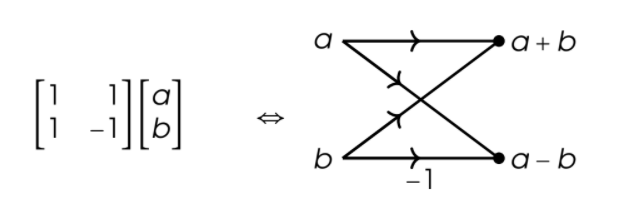
\includegraphics[width=9cm]{EE229 images/Butterfly structure of FFT.png}
    \end{figure}
    \i For integrable $x(t)$ with $y(t)=x'(t)$ as its derivative:
    $$Y(f)=j2\pi f X(f) $$
    \i For $x(t)=c+\tilde{x}(t)$, where $\tilde{x}(t)$ is integrable with derivative $y(t)$:
    $$ \tilde{X}(f) = \frac{Y(f)}{j2\pi f}\hspace{0.05cm} \mathbb{I}_{\{f\hspace{0.05cm}\neq \hspace{0.05cm}0\}} $$
    since $x(t)=c+\tilde{x}(t)$ for some $c\in \mathbb{C}$:
    $$X(f)= \tilde{X}(f) +c\hspace{0.05cm} \delta(f)=\frac{Y(f)}{j2\pi f} +c \hspace{0.05cm}\delta (f) $$
    \i \tb{Z-transform:}
    $$H(z)=\sum_{n\hspace{0.05cm}\in\hspace{0.05cm}\mathbb{Z}} h[n]z^{-n} $$
    polynomial in $z$, which can take complex values
    \i If $x[n]\xrightleftharpoons[]{Z.T.} X(z)$, then $x[n-m]\xrightleftharpoons[]{Z.T.}z_{-m} X(z)$
    \i The DTFT $\hat{X}(f)$ is given by $X(z)$ at $z = e^{(j2\pi f)}$ \i Feedback IIR implementation:
    $$H(z)=\frac{1}{1-az^{-1}}$$
    $$Y(z)(1-az^{-1})=X(z)$$
    $$y[n]-ay[n-1]=x[n]$$
    $$y[n]=x[n]+ay[n-1]~~~\rightarrow~~~{\color{blue}\text{Causal weighted average}}$$
    \begin{figure}[H]
    \centering
    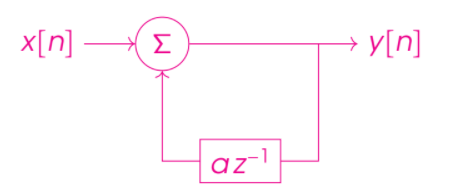
\includegraphics[width=7cm]{EE229 images/Feedback IIR implementation.png}
    \end{figure}
    \i For a frequency response:
    $$\hat{H}(f)=\frac{1}{1-ae^{(-j2\pi f)}},~~~-\frac{1}{2}\leq f\leq \frac{1}{2}$$
    \b{itemize}
        \item[$-$] for $a=1,~~|\hat{H}(f)|=\frac{1}{2 \hspace{0.05cm}sin(\pi f)}~~\rightarrow~~|\hat{H}(f)|=\infty\text{ at } f=0$. The system is not BIBO stable (true for $|a|=1$) 
        \item[$-$] for $a=|a|e^{j\theta},~~|\hat{H}(f)|=\frac{1}{\sqrt{(1+|a|)^2-4|a|\hspace{0.05cm}cos^2(\frac{\theta}{2}+\pi f)}}$. The system is stable for $|a|<1$. For $|a|>1$, the system is BIBO unstable.
    \e{itemize}
\e{itemize}
\e{document}
